Traffic anomaly is detected based on the anomalous fluctuations of queries per second (QPS).
As shown in Figure~\ref{fig:QPS-2-hour} and Figure~\ref{fig:QPS-week}, QPS complies with the normal distribution in both short term and long term.
Therefore, we choose to use the 3-sigma rule to detect anomalous QPS fluctuations.

Similar to performance and reliability anomaly detection, we consider the last 10 minutes as the current detection window.
Based on the QPS values in the last one hour, we use the 3-sigma rule to detect outliers in the current detection window.
To further eliminate false positives, we also check the Pearson correlation coefficient (see Equation~\ref{eq:pearson}) between the QPS values and the business metric values of the initial anomalous service.
Only when the correlation is higher than a predefined threshold (e.g., 0.9) and  3-sigma outliers are identified in the current detection window, a traffic anomaly is reported for the current service.

%\begin{figure}[ht]
%	\centering
%	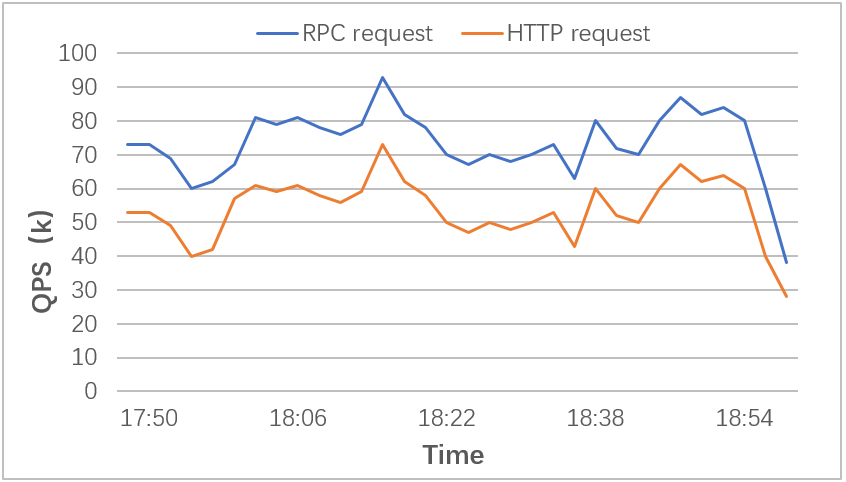
\includegraphics[width=0.45\textwidth]{images/qps-time.png}
%	\vspace{-8pt}
%	\caption{Change of QPS Over Time}\label{fig:qps-time}
%	\vspace{-10pt}
%\end{figure}


